\section{Near-Ballistic Transfers between the Earth-Moon and Sun-Earth Systems}\label{sec:NearBallistic}
While both categories of trajectories travel through the Sun-Earth CR3BP region, only those with an
intermediate staging orbit have a constrained path. For the staging orbit trajectories, the
Earth-Moon unstable manifold arc, propagated under the Sun-Earth CR3BP dynamics once it reaches the
lunar sphere of influence, must intersect with a stable manifold arc from the Sun-Earth staging
$L_{2}$ halo orbit. An unstable manifold arc from the staging orbit is then utilized to depart the
Sun-Earth system (compared to the more direct transfer type that employs the Earth-Moon manifold to
depart the system). Kakoi developed a design methodology for maneuver-free transfers between orbits
in the two systems, treating them as non-coplanar, where the required respective initial
orientations of the three bodies (the Sun, Earth, and Moon) are represented by two angles and the
interface between the CR3BP systems occurs at the intersection of the manifold\
arcs\cite{Kakoi:2014,Kakoi:2015}. Parker and Anderson developed a similar approach utilizing the
Sun-Earth stable and unstable manifolds to design low-energy transfers between Earth and lunar
libration orbits\cite{Parker:2013}. The two previous methodologies inspire the approach employed in
this investigation, where the orientations are determined by a specified epoch date and the two
systems interface before the arc intersection.

\subsection{Methodology}
To find a connection between the orbits in the two different CR3BP systems, discretized arcs of the
manifold surface of the Earth-Moon departure orbit are propagated to the SoI of the Moon, as
defined in \cref{eq:blendedSoI}. At the SoI distance from the Moon, its gravitational influence
becomes negligible compared to those of the Earth and the Sun. At the interface of the two CR3BP
systems, the Earth-Moon barycentric rotating frame state of each arc is transformed to a Sun-Earth
barycentric rotating frame state by rotation to the Earth-centered Ecliptic J2000 frame and back as
described in \cref{sec:FrameTransformations}. The rotation depends on the epoch date when the state
reaches the SoI, determining the relative orientations of the celestial bodies. While the
orientations change slightly month-to-month due to the different planes, the transfer
characteristics tend to repeat each month, so this investigation only analyzes transfers that
depart during January 2026\cite{Parker:2013}. Note that although the SoI intersection states all
have the same Earth-Moon Jacobi constant values, now that they are in the Sun-Earth system, their
Sun-Earth Jacobi constant values vary. Since the new values remain constant as the states are now
propagated with the Sun-Earth CR3BP equations of motion, it is necessary that the Jacobi constant
of the Sun-Earth staging halo orbit lies within that range of Jacoi constant values. The process
ensures that the manifold arcs are seamlessly transitioned between the Earth-Moon and Sun-Earth
CR3BP systems for consistent trajectory analysis.

The manifold arcs are now propagated until they reach the manifold intersection surface, selected
as an angle measured from the $x$-axis in the Sun-Earth rotating frame, centered at the Earth, that
extends as a plane perpendicular to the $xy$-plane. According to Kakoi, plane angles between
$-\ang{85}$ and $\ang{70}$ are desirable for transfers between Earth-Moon $L_{2}$ and Sun-Earth
$L_{2}$ orbits\cite{Kakoi:2015}. In the Earth-centered Sun-Earth rotating frame, the stable
manifolds from the Sun-Earth $L_{2}$ halo orbits utilized in this investigation arrive in the
Earth-Moon vicinity in the fourth quadrant (southeast) that encompasses that range of angles. A
plane angle of $\ang{-80}$ is selected for this investigation. At the same time, the discretized
stable manifold surface from the Sun-Earth $L_{2}$ halo orbit is propagated to the same plane,
appearing in \cref{fig:hyperplane}. The approach ensures that the manifold arcs from both CR3BP
systems align at a common intersection surface, facilitating the identification of potential
transfers.

\begin{figure}[H]
    \centering
    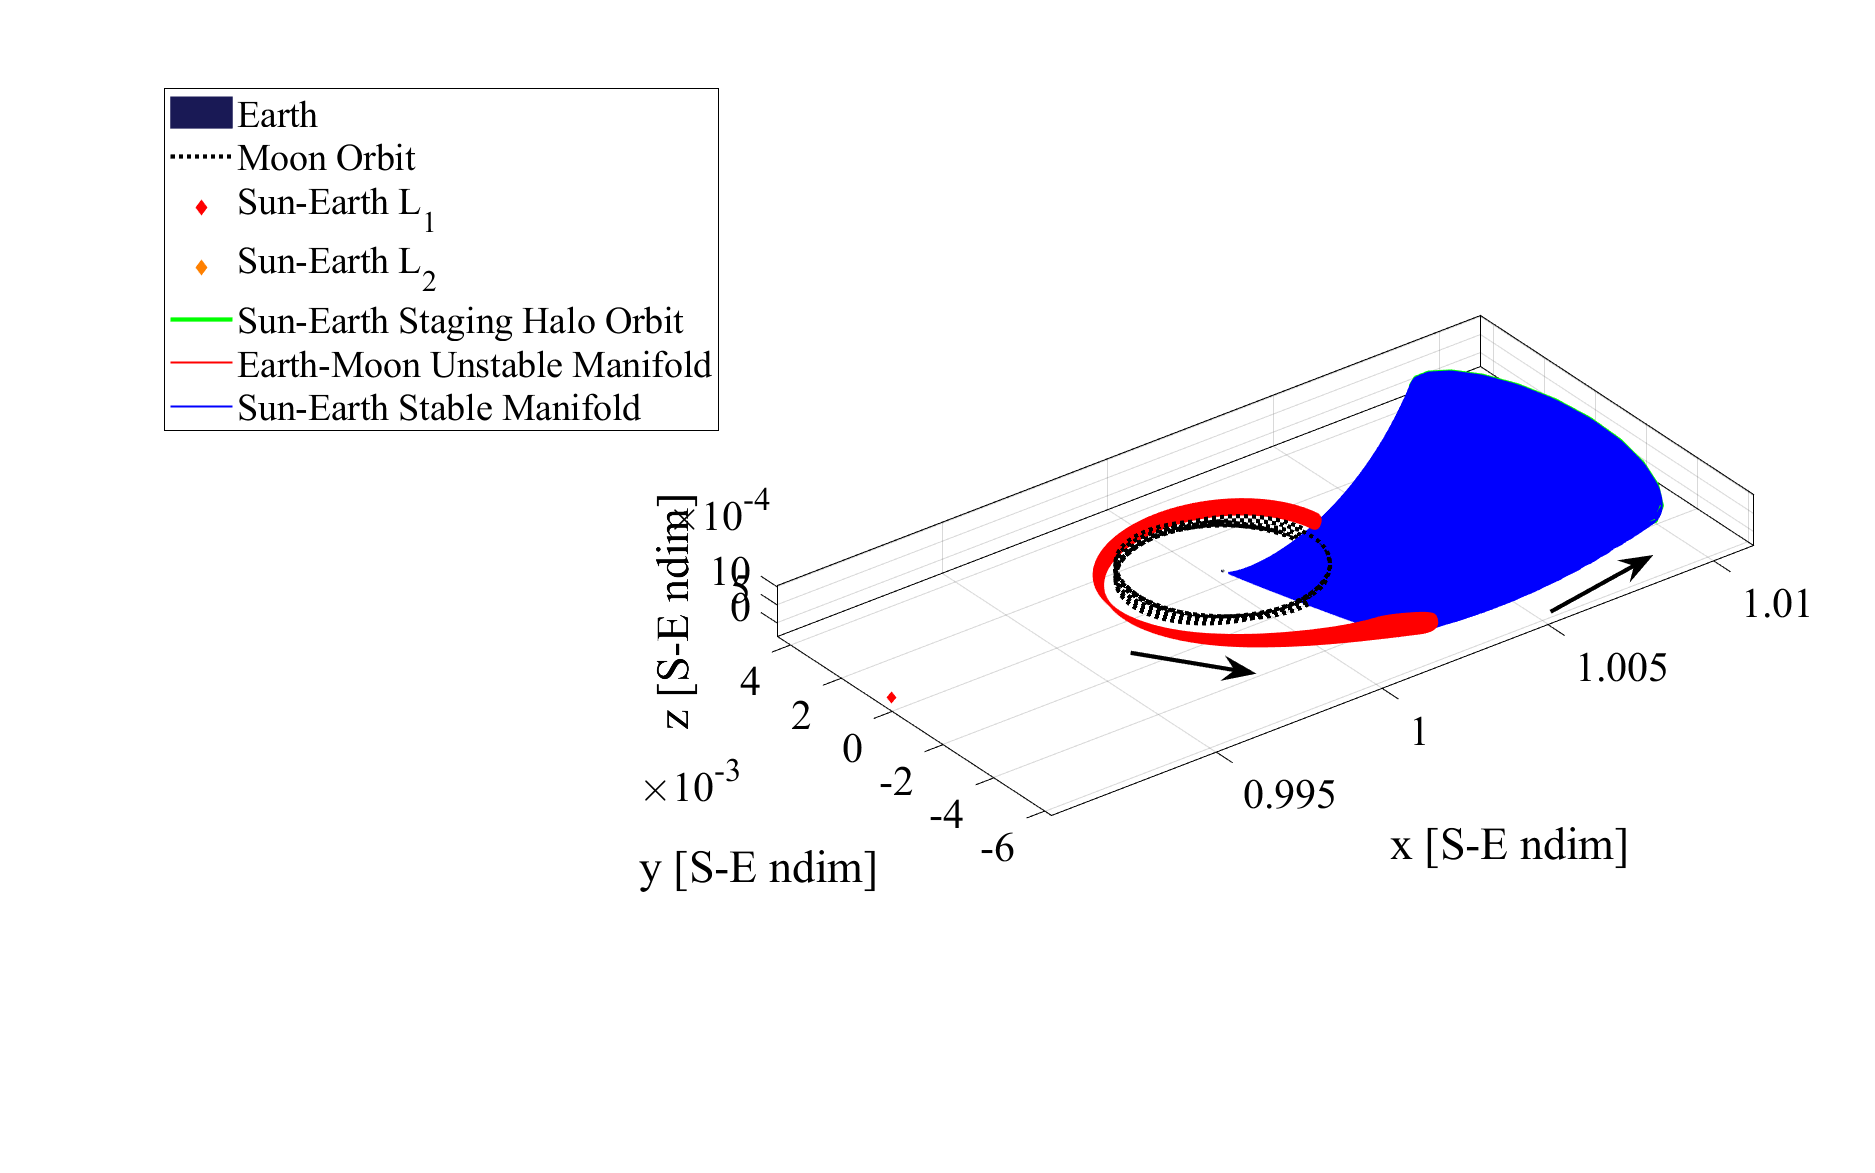
\includegraphics[width=0.9\textwidth]{figures/Hyperplane.pdf}
    \caption{Earth-Moon and Sun-Earth manifolds at the intersection surface in the Sun-Earth rotating frame.}
    \label{fig:hyperplane}
\end{figure}

At the intersection surface, mappings of both manifolds are applied to form phase plots that inform
the transfer initial guess selection. Following Kakoi's approach, the plots represent $\xdot$ vs.
$x$, $z$ vs. $x$, and $\zdot$ vs. $z$. The $y$-value is defined by the $x$-value and the
intersection surface angle, while the $\ydot$-value is determined by the Jacobi
constant\cite{Kakoi:2015}. A black dot along the Earth-Moon manifold curve denotes the arc that
matches the Sun-Earth manifold in Jacobi constant. The two sets of manifold arcs form curves on the
plots and the goal is to find an intersection between the curves that occurs at the black point in
all three phase plots simultaneously. \cref{fig:phasePlots} provides an example of the phase plots,
where the red curve is the unstable Earth-Moon manifold arcs and the blue curve is the stable
Sun-Earth manifold arcs. Note that there are two black markers representing two individual arcs
that match the Sun-Earth Jacobi constant. The phase plots provide a clear visualization of
potential transfer connections and serve as a critical tool for identifying initial guesses that
satisfy the required dynamical conditions.

\begin{figure}[H]
    \centering
    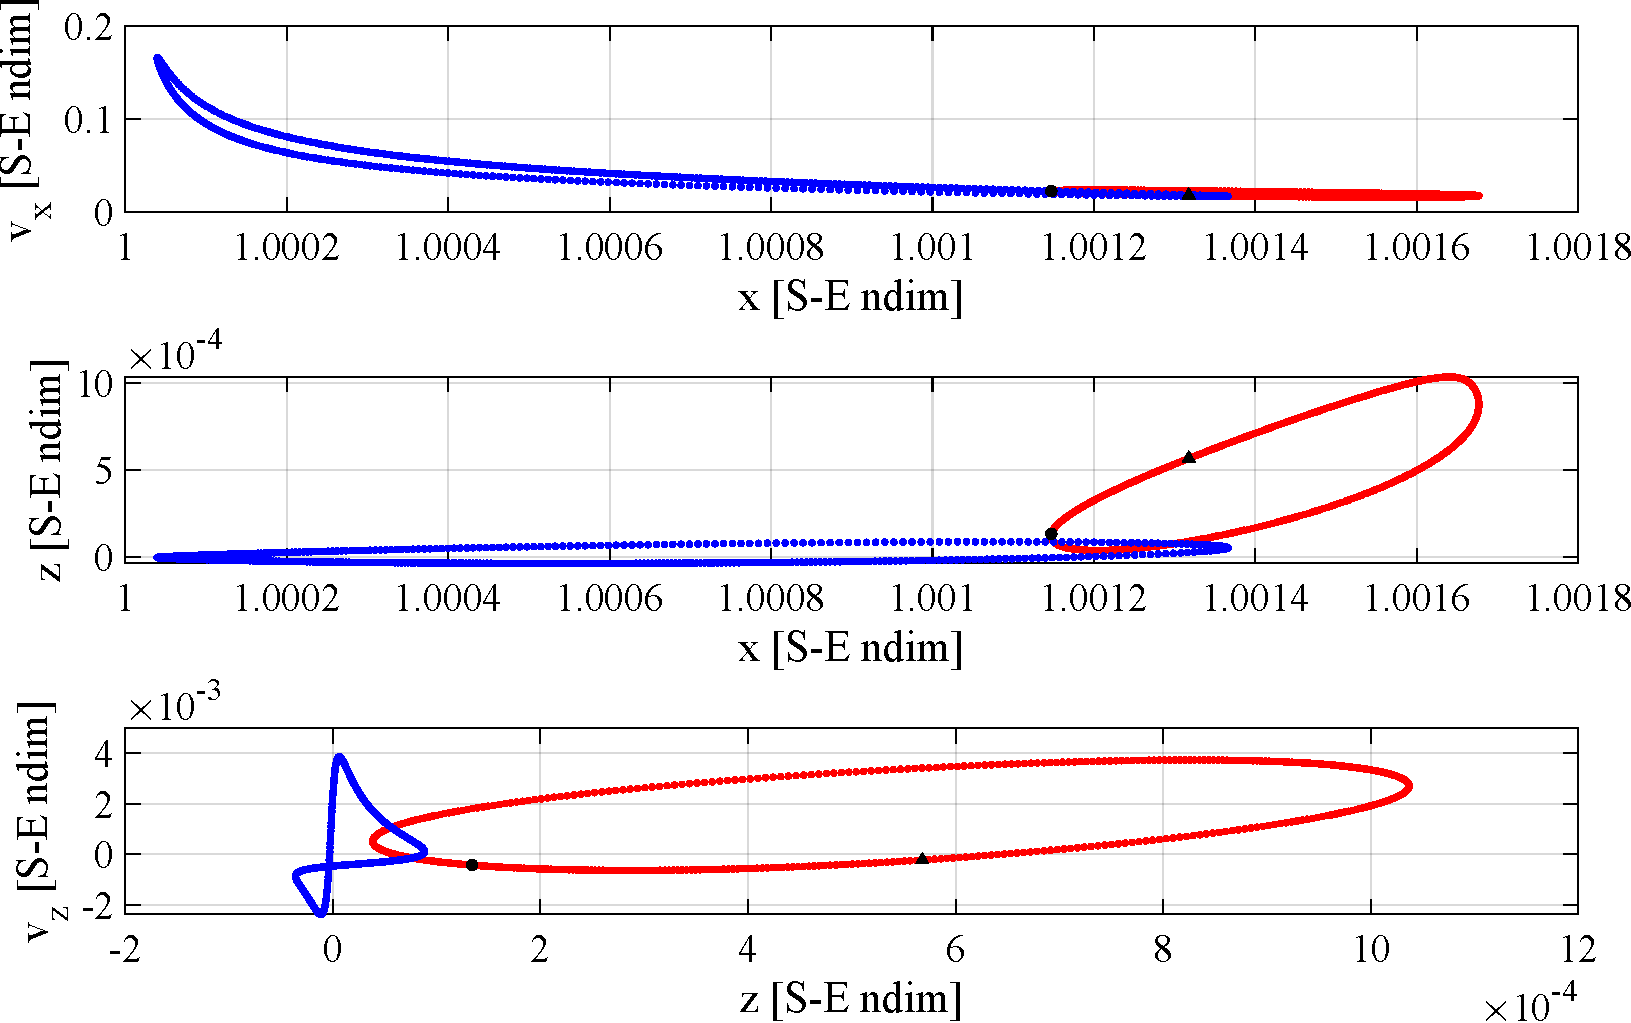
\includegraphics[width=0.75\textwidth]{figures/PhasePlots.pdf}
    \caption{The intersection surface phase plots for \cref{fig:hyperplane}.}
    \label{fig:phasePlots}
\end{figure}

The initial epoch of the Earth-Moon manifold departure, the intersection surface angle, and the
Sun-Earth halo orbit Jacobi constant are all varied to shift the curves on the phase plots and find
an intersection; Kakoi provides some guidelines for doing so\cite{Kakoi:2015}. Once a suitable
point is determined, like the black circle marker in \cref{fig:phasePlotsIntersect}, the resulting
information is utilized to generate an initial guess for the transfer between the systems,
appearing in \cref{fig:initialGuess}. The initial guess is then corrected to find a position
intersection (a maneuver is allowed at the intersection) employing an iterative Newton-Raphson
scheme:
\begin{equation}
    \Xbar=\begin{bmatrix}   T_{0}   &   \tau_{1}    &   t_{1}   &   \tau_{2}    &   t_{2}   \end{bmatrix}^{T},
    \label{eq:nbfreevar}
\end{equation}
\vspace{1mm}
\begin{equation}
    \Fbar(\Xbar)=\begin{bmatrix}    \rbar_{2}-\rbar_{1} &   ||\vbar_{2}-\vbar_{1}|| \end{bmatrix}^{T}.
    \label{eq:nbconst}
\end{equation}
where $T_{0}$ is the initial epoch, $\tau_{1}$ and $\tau_{2}$ are the phase along the Earth-Moon
and Sun-Earth orbits where the manifold steps-off, respectively, $t_{1}$ and $t_{2}$ are the
times-of-flight along each manifold arc, $\rbar_{1}$ and $\rbar_{2}$ are the manifold arc positions
at the end of the propagation, and $\vbar_{1}$ and $\vbar_{2}$ are the velocity vectors at those
points, respectively. The central difference method from \cref{sec:DifferentialCorrections} is
applied to determine the $DF$ Jacobian matrix. Note that the magnitude of the maneuver is included
as the second constraint in the targeting problem. For the first implementation of the targeter,
the $\Delta v$ of the initial guess is the constraint value. Then, each time a solution is
converged, the constraint value is decreased and the targeting problem is repeated to find a
near-ballistic solution with a local minimum in $\Delta v$. Also note that during the process, the
intersection location of the two manifold arcs is free to shift from the designated intersection
surface. The result of the process is a near-ballistic transfer between an Earth-Moon orbit and a
Sun-Earth halo orbit utilizing their invariant manifolds. The transfers have low maneuver costs
that are often absorbed by the dynamics once the solution is transferred to a higher-fidelity
dynamical model. The iterative process ensures the generation of efficient transfer trajectories
with minimal $\Delta v$, serving as a robust foundation for preliminary transfer design.

\subsection{Example}
As an example, consider the phase plots in \cref{fig:phasePlotsIntersect} and the resulting initial
guess in \cref{fig:initialGuess}. The unstable manifold arc departs from an Earth-Moon $L_{2}$
northern halo orbit with an Earth-Moon Jacobi constant of $3.13$ on January 2, 2026 at 07:12:00,
while the stable manifold arc arrives at a Sun-Earth northern halo orbit with a Sun-Earth Jacobi
constant of $3.0008189$. At the intersection surface, the two arcs have a position discontinuity of
$8.768\times10^{-6}$ Sun-Earth nondimensional units ($1312$ km) and a $\Delta v$ of $57.4$ m/s. The
iterative corrections process outlined above produces a position continuous trajectory with a
$\Delta v$ of $14.6$ m/s, a negligible amount in comparison to the rest of the end-to-end transfer.
The initial departure epoch has also shifted slightly, to January 2, 2026 at 07:32:35. The
corrected trajectory appears in \cref{fig:solution}. Note that the location of the maneuver has
shifted from the defined intersection surface to earlier along the Earth-Moon manifold arc. While
this exact solution is only available for the given epoch, every month a similar solution presents
itself, so this represents potential near-ballistic transfer solutions in every month. The
example highlights the effectiveness of the iterative corrections process in refining initial
guesses into near-ballistic transfer solutions.
\vspace{45mm}

\begin{figure}[H]
    \centering
    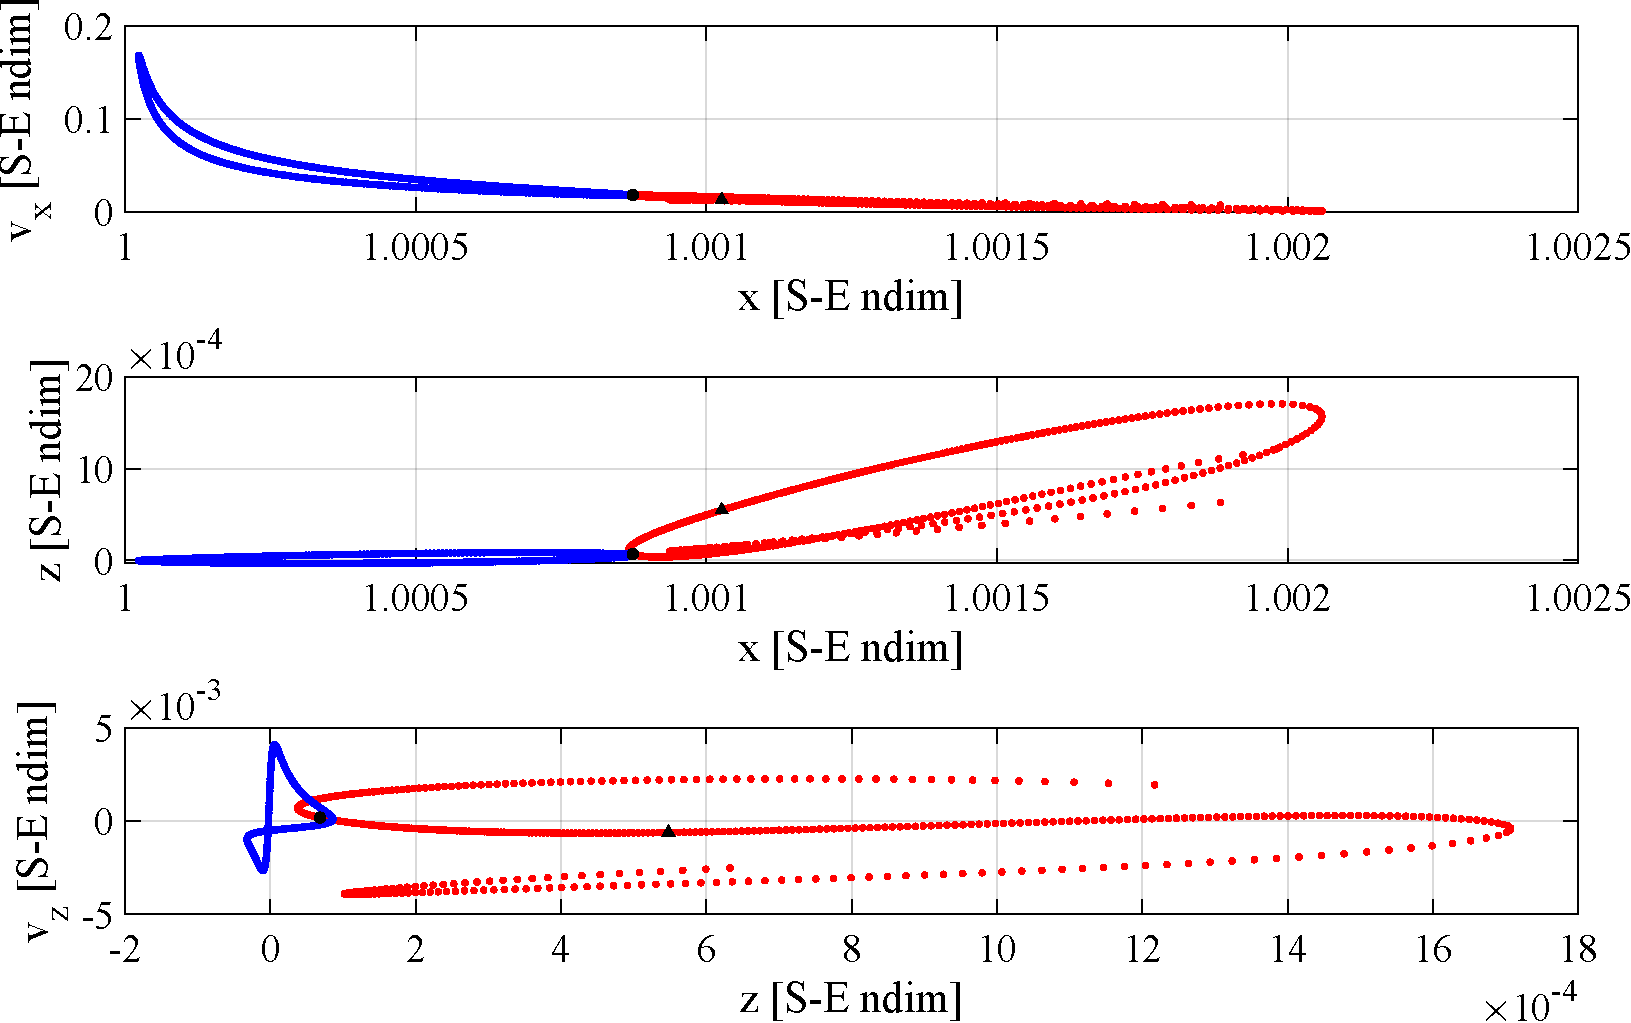
\includegraphics[width=0.75\textwidth]{figures/PhasePlotsIntersect.pdf}
    \caption{Intersection surface phase plots with a near intersection after varying the parameters.}
    \label{fig:phasePlotsIntersect}
\end{figure}

\begin{figure}[H]
    \centering
    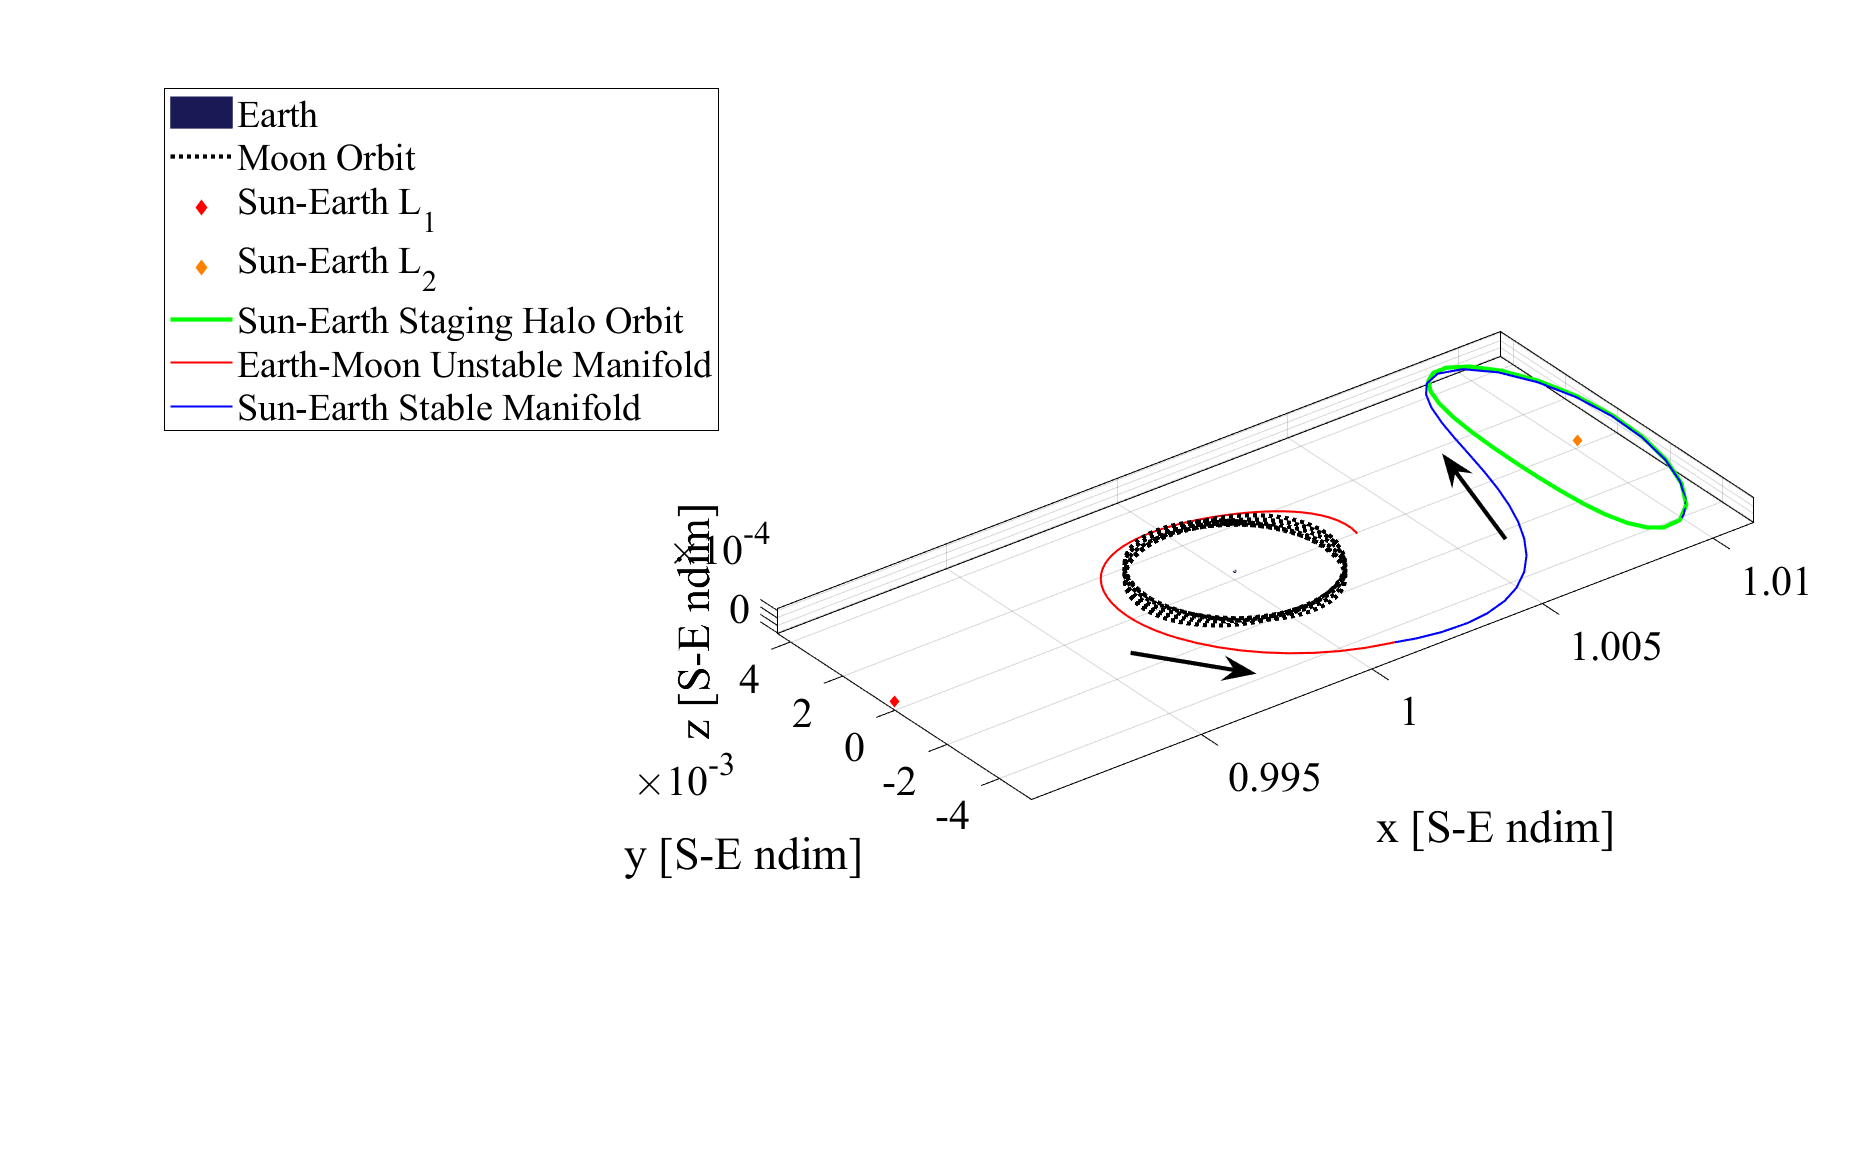
\includegraphics[width=0.9\textwidth]{figures/InitialGuess.pdf}
    \caption{Initial guess for near-ballistic Earth-Moon to Sun-Earth transfer from phase plots in the Sun-Earth rotating frame.}
    \label{fig:initialGuess}
\end{figure}

\begin{figure}[H]
    \centering
    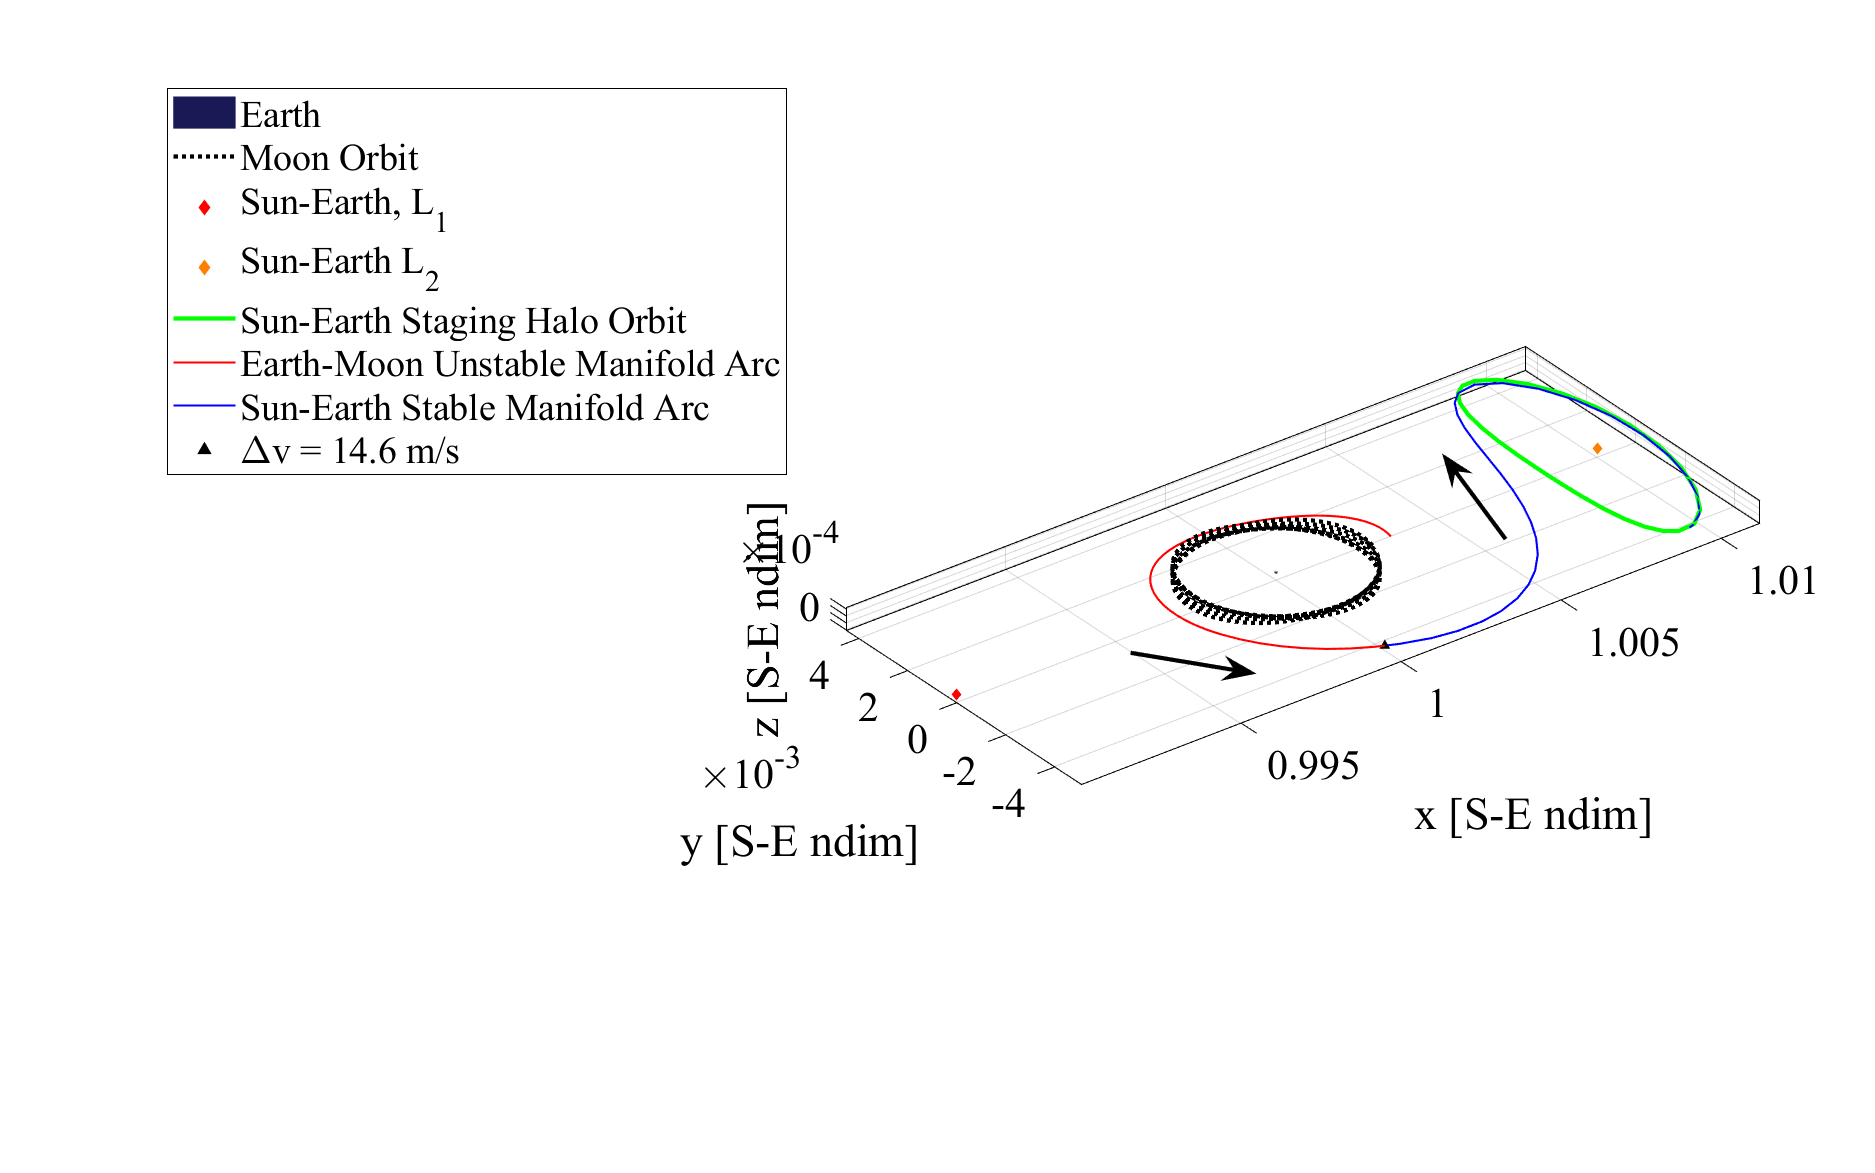
\includegraphics[width=0.9\textwidth]{figures/Solution.pdf}
    \caption{Converged near-ballistic tranfer between Earth-Moon and Sun-Earth halo orbits in the Sun-Earth rotating frame.}
    \label{fig:solution}
\end{figure}
